\documentclass[11pt,a4paper]{article}
\usepackage[margin=22mm]{geometry}
\usepackage[T1]{fontenc}
\usepackage{lmodern,graphicx,booktabs,tabularx,array,xurl,microtype,amsmath}
\usepackage[dvipsnames]{xcolor}
\usepackage[hidelinks]{hyperref}
\usepackage{fancyhdr}
\definecolor{macrogreen}{HTML}{23734B}
\graphicspath{{figures/}{../figures/}}
\setlength{\parindent}{0pt}
\setlength{\parskip}{6pt}
\setlength{\emergencystretch}{3em}
\renewcommand{\topfraction}{0.9}
\renewcommand{\bottomfraction}{0.9}
\renewcommand{\textfraction}{0.1}
\renewcommand{\floatpagefraction}{0.8}
\setcounter{topnumber}{3}
\setcounter{totalnumber}{4}
\pagestyle{fancy}\fancyhf{}
\fancyhead[L]{\small\textcolor{macrogreen}{MACROMATE}}
\fancyhead[R]{\small Final technical report}
\fancyfoot[C]{\small\thepage}
\setlength{\headheight}{14pt}
\newcommand{\code}[1]{\texttt{\detokenize{#1}}}
\begin{document}
\hypersetup{pageanchor=false}
\begin{titlepage}
\vspace*{20mm}
{\color{macrogreen}\large DELIVERABLE 3\par}
\vspace{8mm}
{\Huge\bfseries MacroMate\par}
\vspace{4mm}
{\LARGE Image-assisted meal recognition\\and nutrition logging\par}
\vspace{12mm}
{\large Data preparation, model evaluation, and application integration\par}
\vspace{16mm}
\begin{tabular}{ll}
Hassan Mehmood & 24L-2559\\
Mohid Israr & 24L-2510\\
Adnan Zaka & 24i-2537
\end{tabular}
\vfill
Repository: \url{https://github.com/MhassaanK68/macromate}\\
Prepared: 20 November 2026\\
Live app: \url{https://macromate-nu.vercel.app}
\end{titlepage}
\hypersetup{pageanchor=true}
\pagenumbering{roman}

\begin{abstract}
MacroMate combines an eight-class food recognizer with a manually confirmed,
reference-based nutrition workflow. The collection contains 400 photographs,
balanced at 50 per dish, with a group-aware 280/64/56 train/validation/test split.
A partially fine-tuned CLIP ViT-B/32 updates the last two vision blocks, final
vision normalization, and visual projection while retaining frozen text features.
The recorded experiment selected epoch 6 from 11 epochs and classified 54 of 56
held-out photos correctly (96.43\%); top-three accuracy was 56/56 and macro F1
was 0.9641. These are historical experimental results, not accuracy measurements
of arbitrary user uploads. The new Python application validates uploaded images,
shows ranked suggestions, requires explicit dish confirmation, scales nutrition
by user-entered grams, and supports a temporary daily log with CSV export.
Model assets are provisioned with integrity checks. Software validation and
deployment status are reported separately from model evaluation. The small,
source-confounded test set, unsupported unfamiliar foods, recipe proxies, and
temporary storage limit practical use.
\end{abstract}
\begingroup\small\tableofcontents\endgroup
\clearpage
\pagenumbering{arabic}

\section{Introduction and scope}
Logging familiar meals often requires finding a dish name, estimating a serving,
and looking up nutrition manually. MacroMate reduces the label-search step while
leaving two decisions with the user: which dish was actually eaten and how many
grams were served. Recognition ranks eight labels; it does not infer ingredients,
food weight, or personalized dietary needs.

Supported labels are chicken biryani, chicken pulao, chicken karahi, daal, nihari,
haleem, samosa, and chapati. A photo should show one supported main dish. Mixed
plates, automatic portion estimation, user accounts, persistent health records,
and medical recommendations are outside the implemented scope.

This report integrates the data work from Deliverable 1, the model and recorded
evaluation from Deliverable 2, and the application work from Deliverable 3. The
selected implementation route is application development (Track A). The application's
software tests do not replace held-out model evaluation or prove public-host readiness.

\section{Related work and design choice}
CLIP learns an image--text embedding space and permits text-described categories
to be compared with visual features~\cite{clip}. The underlying Vision Transformer
represents an image as patch tokens processed through self-attention~\cite{vit}.
This supports reusing a pretrained visual representation for a small dataset
instead of training a large recognizer from scratch.

MacroMate uses fixed prompts of the form ``a photo of Pakistani [dish]'' and
partially adapts the vision encoder. The limited dataset motivated this restricted
training scope; it does not prove that this architecture is optimal. The initial
proposal discussed a zero-shot comparison, but this report makes no new
zero-shot-versus-fine-tuned test claim. The final application route reuses the
existing evaluated checkpoint without selecting new thresholds on the test set.

Streamlit provides a Python interface directly around the recognizer, avoiding a
separate API server for this prototype. Its AppTest tooling supports simulated
widget interactions~\cite{streamlit-test}. Hosting targets Vercel's Python/ASGI
runtime~\cite{vercel}, with Community Cloud as an alternative~\cite{streamlit-cloud}.

\section{Data collection, preparation, and provenance}
\subsection{Collection and sources}
The committed collection has 400 images, 50 for each class. Four public Roboflow
Universe sources supply the selected images. Source URLs, original labels,
transformations, image identities, and uploader-stated CC BY 4.0 attribution are
retained in \code{data/sources.csv} and \code{data/metadata.csv}.

\begin{center}
\begin{tabularx}{\linewidth}{Xr}
\toprule Source & Selected images\\\midrule
combined-dataset, Rafias Workspace & 258\\
IndianFoodRecog, EnVisionAI & 64\\
samosa, uploader ``new'' & 50\\
Bangladeshi Food Classification2, NSN & 28\\
\bottomrule
\end{tabularx}
\end{center}
Original provider archives and README files were not retained; their recorded
archive hashes and uploader license statements cannot be independently rechecked
against original exports. A second independent human label review remains pending.
Regional label mappings, including morog polao to chicken pulao and multiple daal
variants, remain documented limitations.

\subsection{Cleaning and preprocessing}
The recorded cleaning checks found no missing records, unreadable images, unknown
labels, duplicate IDs, exact duplicates, or conflicting exact-duplicate labels.
All 400 records were retained. A 64-bit difference-hash threshold of six bits
flagged no near-duplicate pair; the minimum distance was ten bits. Six groups
derived from the same source photographs were kept within a single split.
Four high-file-size outliers were visually retained rather than automatically removed.

Preprocessing corrects EXIF orientation, converts to RGB, resizes the shorter side
to 224 pixels with bicubic interpolation, and center-crops to $224\times224$.
Prepared RGB PNGs are scaled by $1/255$ and normalized once at model input using
CLIP means $(0.48145466,0.4578275,0.40821073)$ and standard deviations
$(0.26862954,0.26130258,0.27577711)$. Uploads use this same model pipeline; the
UI does not implement a second normalization path.

\subsection{Split and exploratory analysis}
The seeded, group-aware split uses 35 training, eight validation, and seven test
images per class: 280/64/56 overall (70\%/16\%/14\% after integer allocation).
Recorded checks found no group or near-duplicate leakage across splits. Two full
preparation runs produced 424 identical generated outputs.

\begin{figure}[htbp]\centering
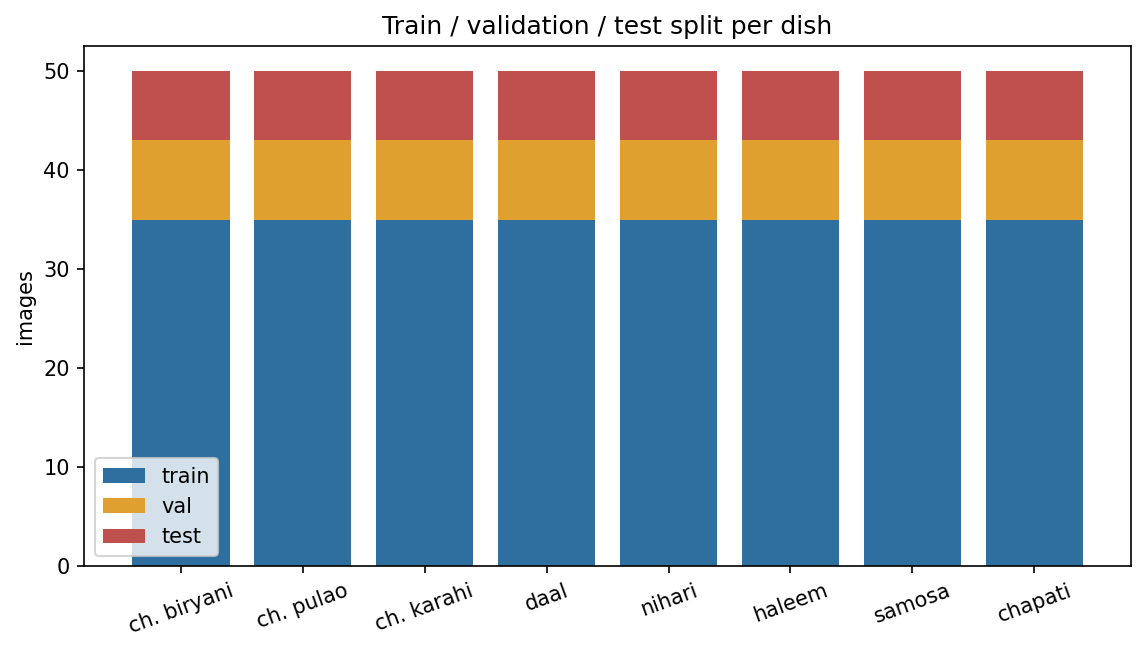
\includegraphics[width=.83\linewidth]{split_distribution.png}
\caption{Recorded data split, with seven held-out test photos per dish. Counts describe
the prepared collection, not a new application experiment.}
\end{figure}

Source resolution and class are correlated: chapati and samosa mainly use 640-pixel
single-source images, several dishes use 432-pixel images, and part of pulao uses
256-pixel images. Provider stretching makes all committed images square. Resizing
does not remove background, style, source, or regional confounding.

\begin{figure}[htbp]\centering
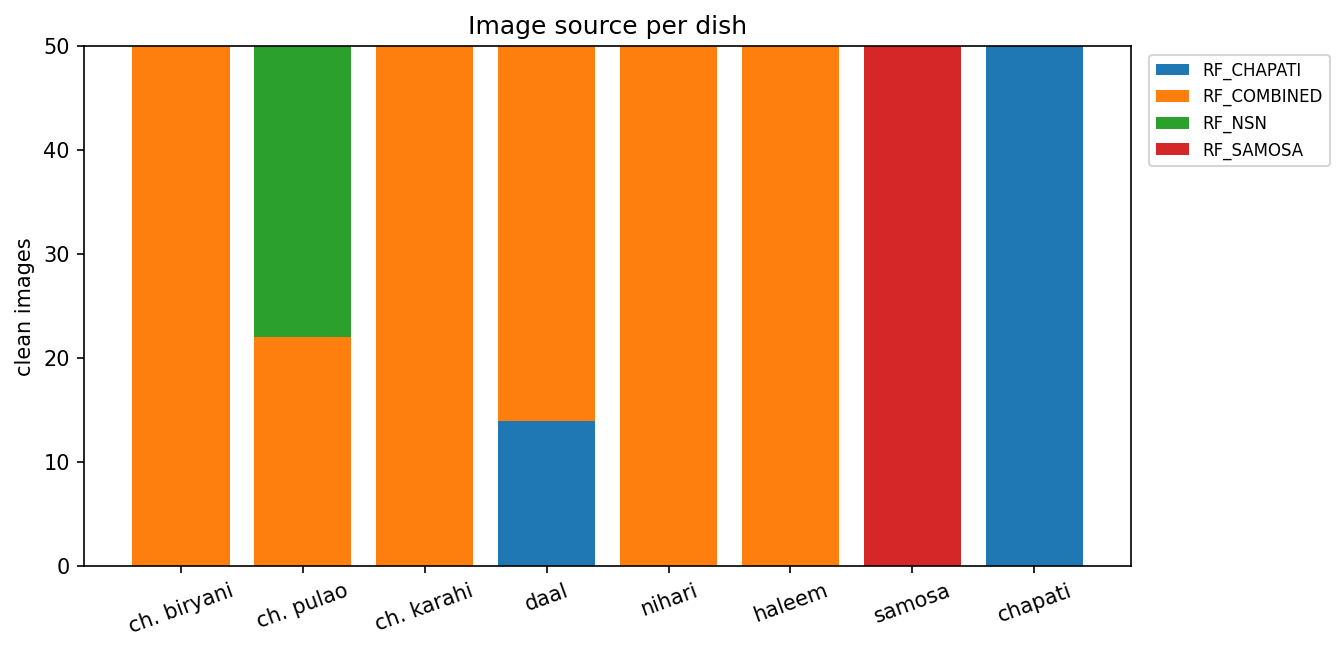
\includegraphics[width=.84\linewidth]{class_by_source.png}
\caption{Recorded class/source distribution. Single-source classes make source style
a possible shortcut. Source attribution is retained in the manifests.}
\end{figure}

\section{Model architecture and training}
CLIP ViT-B/32 uses 49 image-patch tokens plus a class token for a $224\times224$
image, vision hidden width 768, 12 Transformer blocks, 12 attention heads, and
3072-wide feed-forward layers. The class-token output passes through final layer
normalization and a 768-to-512 projection. The text encoder produces fixed,
normalized 512-dimensional vectors for the eight prompts.

For image embedding $v$ and prompt embedding $t_c$, the class logit is
\begin{equation}
z_c=\exp(s)\,\frac{v}{\|v\|}\mathbin{\cdot}\frac{t_c}{\|t_c\|},
\end{equation}
where $s$ is CLIP's logit-scale parameter. Softmax scores rank only the supported
classes; they are uncalibrated and provide no unfamiliar-food rejection.

\begin{figure}[htbp]\centering
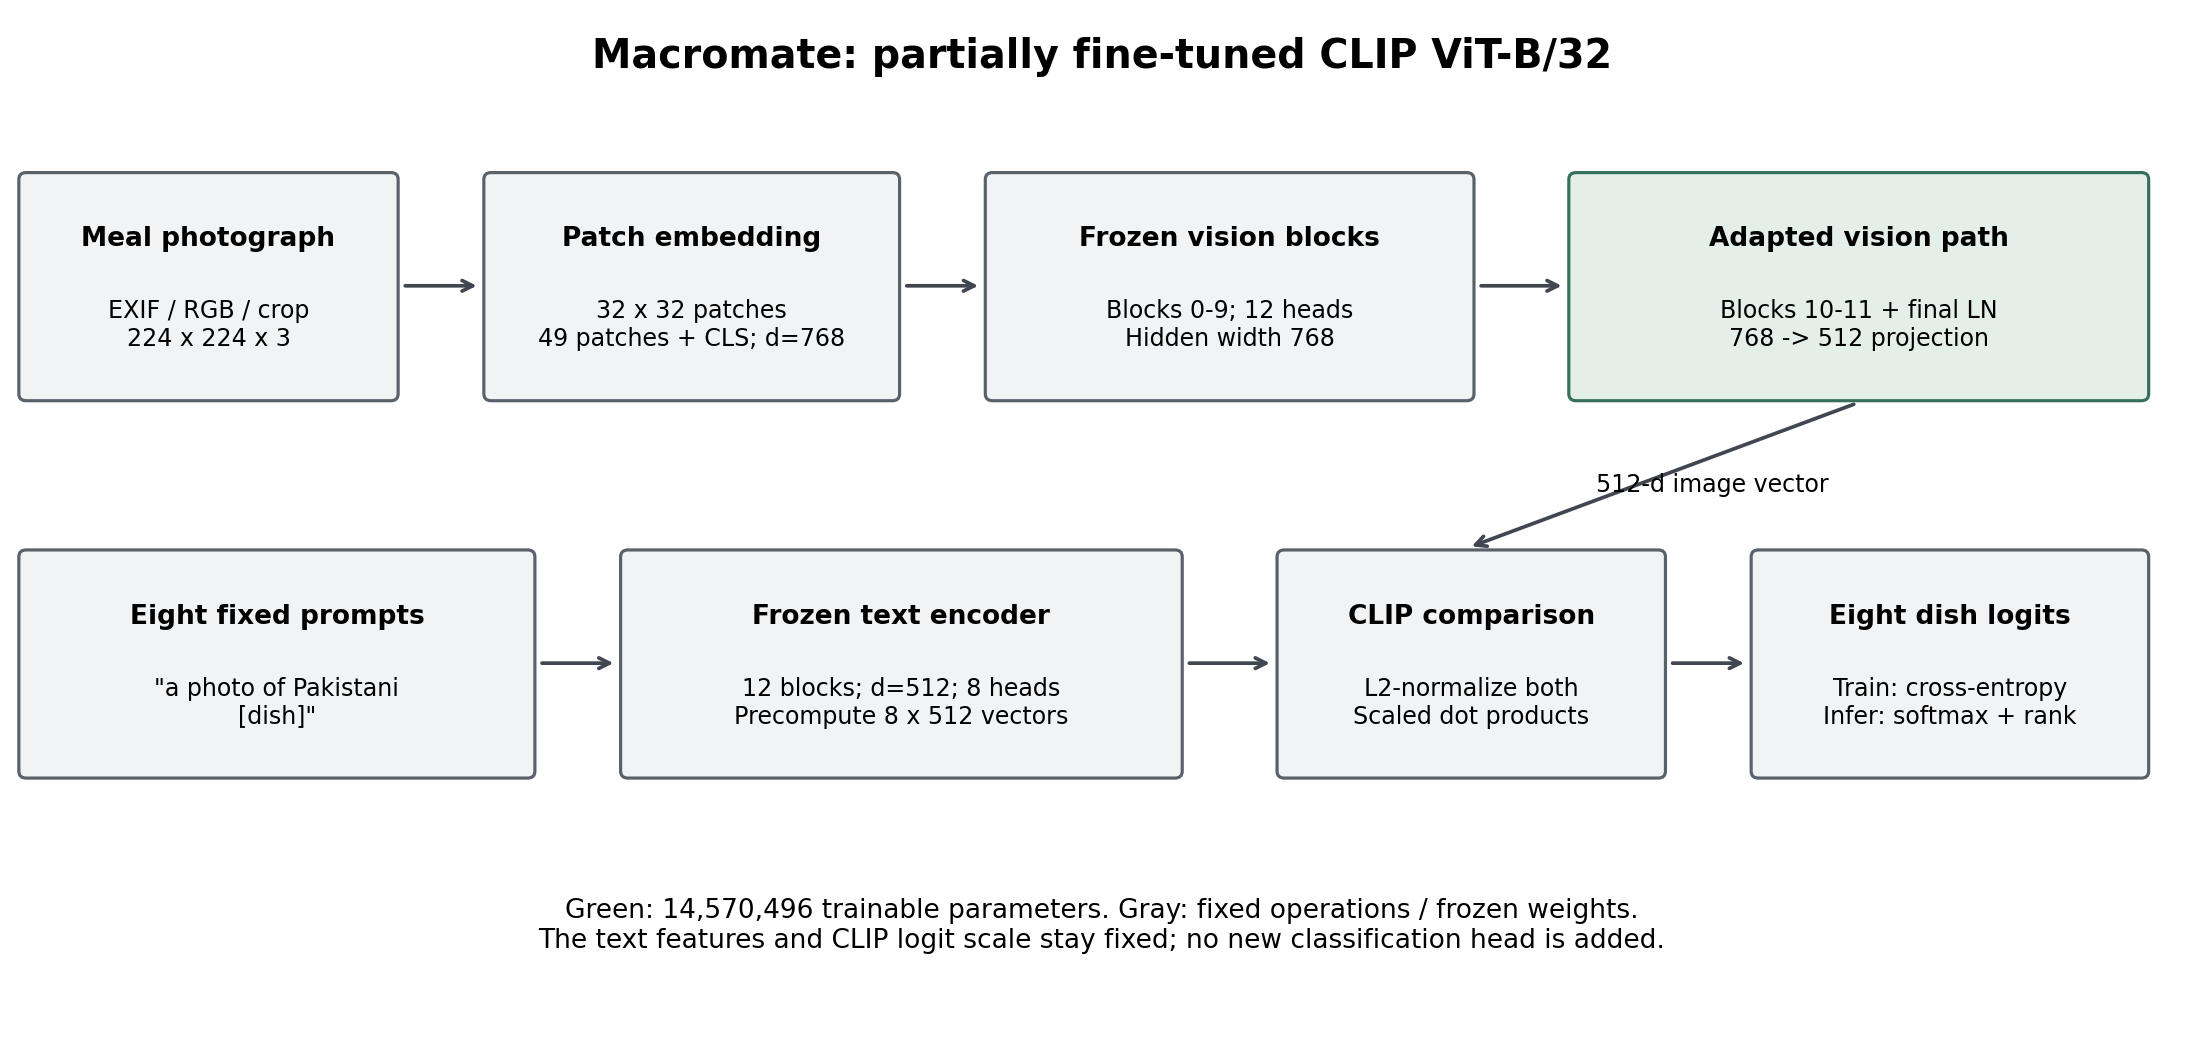
\includegraphics[width=.96\linewidth,height=.37\textheight,keepaspectratio]{model/architecture.png}
\caption{Recorded model architecture and fine-tuning paths. No new classification head
or model architecture is introduced for the application.}
\end{figure}

Only vision blocks 10 and 11, final vision layer normalization, and the visual
projection are updated (14,570,496 trainable parameters). The text side remains
frozen. The base is pinned to revision
\path{3d74acf9a28c67741b2f4f2ea7635f0aaf6f0268}.

\begin{center}\begin{tabularx}{\linewidth}{Xl}
\toprule Setting & Recorded value\\\midrule
Loss & Categorical cross-entropy\\
Optimizer & AdamW; betas 0.9/0.999; epsilon $10^{-8}$\\
Vision-block learning rate & $2\times10^{-5}$\\
Norm/projection learning rate & $5\times10^{-5}$\\
Batch size / weight decay & 8 / 0.01\\
Scheduler / clipping & 10\% warmup then cosine / norm 1.0\\
Maximum epochs / patience / seed & 20 / 5 / 42\\
Selected / executed epoch counts & 6 / 11\\
\bottomrule\end{tabularx}\end{center}

Biases and normalization parameters receive no weight decay. There are no class
weights, label smoothing, or added dropout. The historical six-candidate,
two-epoch pilot compared baseline, lower/higher block learning rates, a lower
projection learning rate, batch 16, and no decay. The higher block-rate candidate
was selected at 58/64 validation correct with the lowest tied-count loss
(0.282456). These short, single-seed pilots do not establish a global optimum.

The full run selected the highest validation correct count, then lower loss,
retaining an earlier epoch for exact ties. Epoch 6 achieved 61/64 validation
top-one (95.31\%), 64/64 top-three, and loss 0.215961. Five epochs without
improvement stopped training after epoch 11.

\begin{center}\footnotesize
\begin{tabularx}{\linewidth}{Xrrrrrr}
\toprule Pilot & Block LR & Proj. LR & Batch & Decay & Correct & Loss\\\midrule
Baseline & $10^{-5}$ & $5\times10^{-5}$ & 8 & .01 & 58/64 & .294529\\
Block low & $5\times10^{-6}$ & $5\times10^{-5}$ & 8 & .01 & 57/64 & .307729\\
Block high & $2\times10^{-5}$ & $5\times10^{-5}$ & 8 & .01 & 58/64 & .282456\\
Projection low & $10^{-5}$ & $2\times10^{-5}$ & 8 & .01 & 57/64 & .302356\\
Batch 16 & $10^{-5}$ & $5\times10^{-5}$ & 16 & .01 & 57/64 & .344546\\
No decay & $10^{-5}$ & $5\times10^{-5}$ & 8 & 0 & 58/64 & .294530\\
\bottomrule\end{tabularx}\end{center}
All pilot measurements above are recorded validation results, not new Deliverable 3 experiments.

\begin{figure}[htbp]\centering
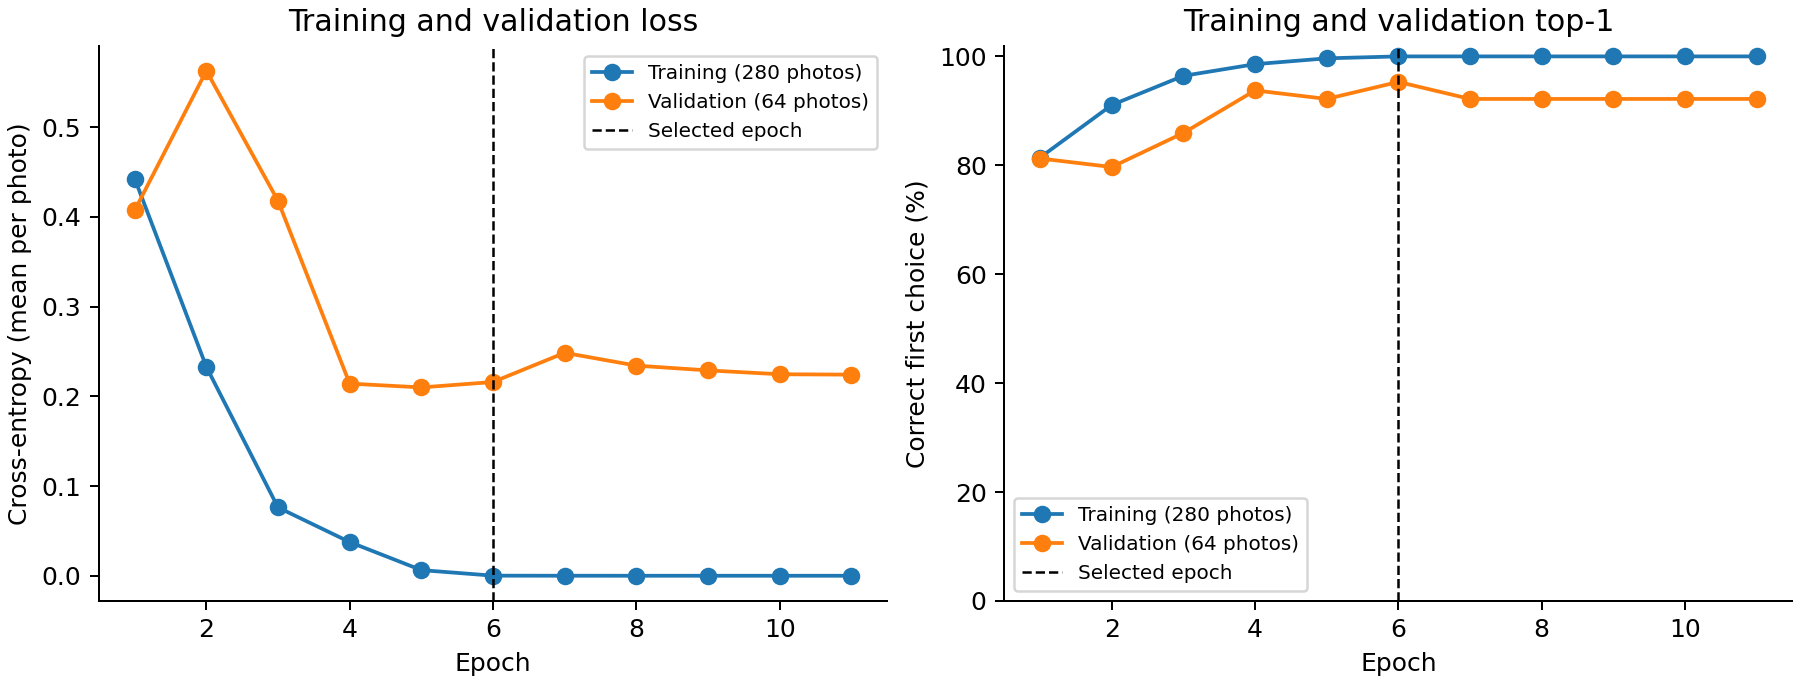
\includegraphics[width=.95\linewidth]{model/learning_curves.png}
\caption{Training and validation history from saved Deliverable 2 evidence. Epoch 6
is the selected checkpoint; application development did not retrain it.}
\end{figure}

\section{Recorded evaluation and discussion}
The held-out results come from \code{evidence/predictions.csv} and
\code{evidence/evaluation.json}. Counts and aggregate metrics describe the same
56-photo test set; they do not measure arbitrary phone uploads.

\begin{center}\begin{tabularx}{\linewidth}{Xr}
\toprule Metric & Recorded result\\\midrule
Top-one correct & 54/56 (96.43\%)\\
Top-three correct & 56/56 (100\%)\\
Macro F1 & 0.9641\\
Macro one-vs-rest ROC-AUC & 0.9985\\
Test examples per class & 7\\
\bottomrule\end{tabularx}\end{center}

\begin{center}\small
\begin{tabularx}{\linewidth}{Xrrrr}
\toprule Dish (support 7 each) & Precision & Recall & F1 & ROC-AUC\\\midrule
Chicken biryani & 1.0000 & 1.0000 & 1.0000 & 1.0000\\
Chicken pulao & 1.0000 & 1.0000 & 1.0000 & 1.0000\\
Chicken karahi & 0.8750 & 1.0000 & 0.9333 & 0.9942\\
Daal & 1.0000 & 1.0000 & 1.0000 & 1.0000\\
Nihari & 1.0000 & 0.8571 & 0.9231 & 0.9942\\
Haleem & 1.0000 & 0.8571 & 0.9231 & 1.0000\\
Samosa & 1.0000 & 1.0000 & 1.0000 & 1.0000\\
Chapati & 0.8750 & 1.0000 & 0.9333 & 1.0000\\\midrule
Macro / support-weighted & 0.9688 & 0.9643 & 0.9641 & 0.9985\\
\bottomrule\end{tabularx}\end{center}
Precision measures true positives among predicted positives; recall measures
true positives among actual positives. F1 is their harmonic mean. Macro averages
weight dishes equally, and support-weighted means coincide here because support
is balanced. ROC-AUC measures one-vs-rest ranking across thresholds, not calibration.

\begin{figure}[htbp]\centering
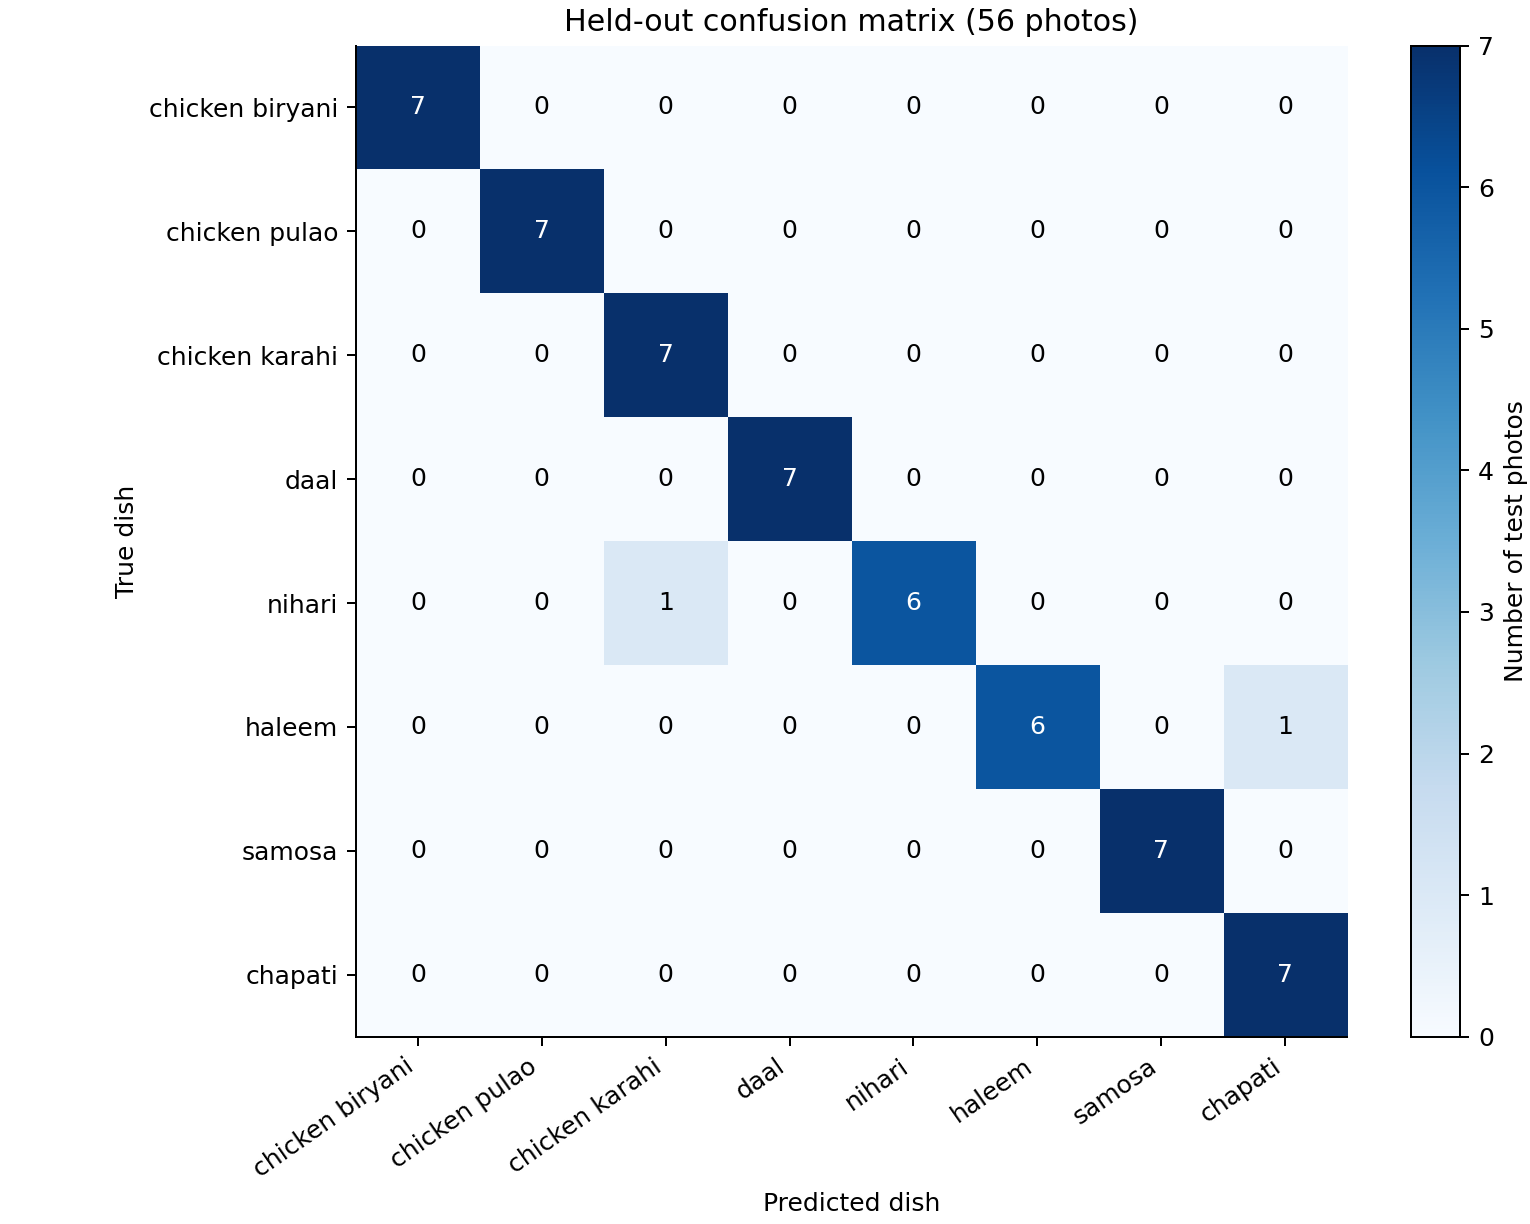
\includegraphics[width=.72\linewidth]{model/confusion_matrix.png}
\caption{Recorded held-out confusion matrix. Rows represent true labels and columns
predicted labels; the test set contains seven examples per class.}
\end{figure}

The two errors were nihari ranked first as chicken karahi and haleem ranked first
as chapati. The correct dish was second in both cases. These examples motivate
showing three suggestions and allowing correction, but this UI choice does not
establish improved classifier accuracy.

\begin{figure}[htbp]\centering
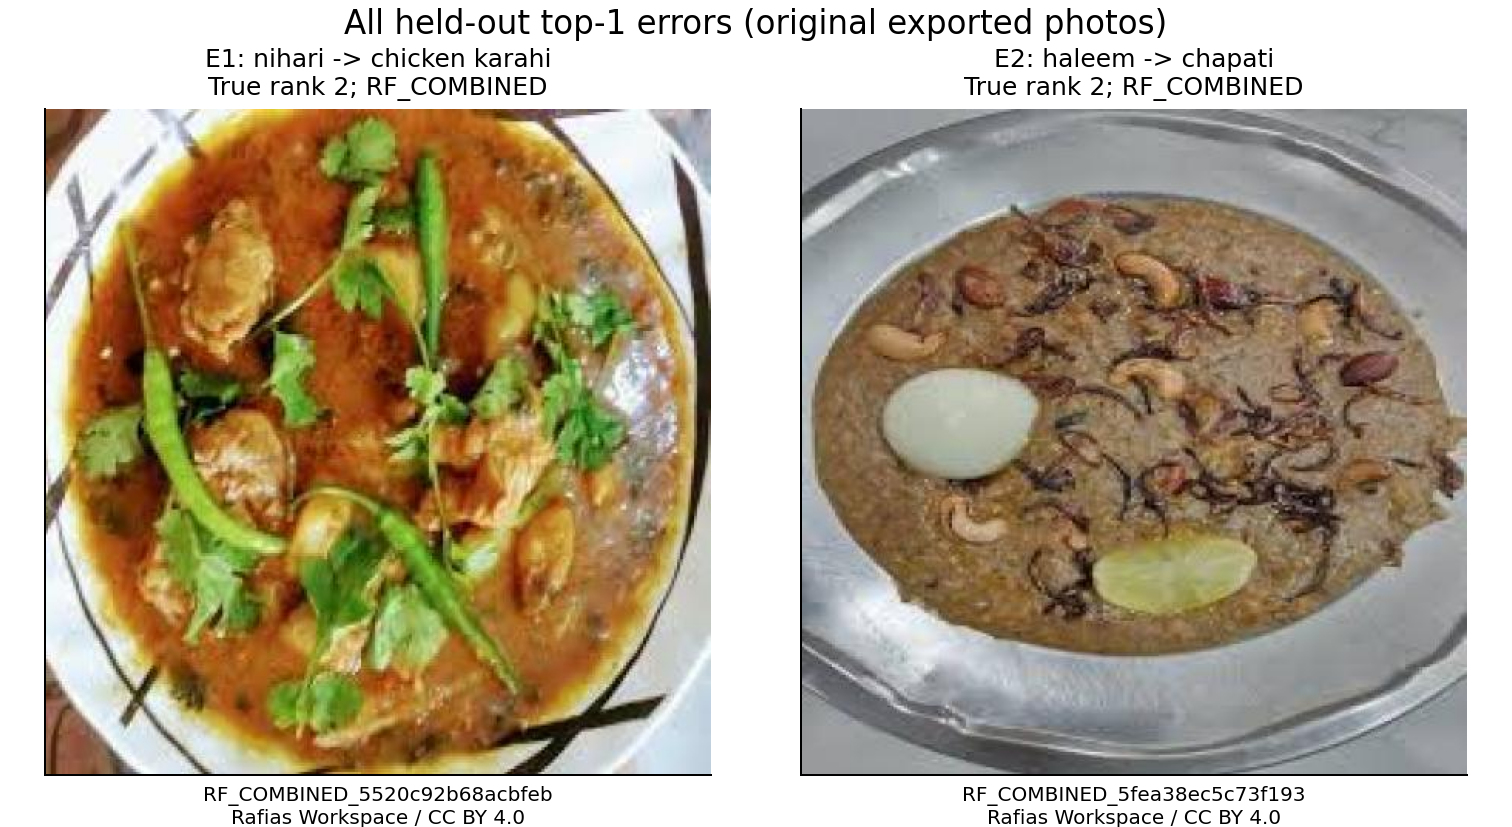
\includegraphics[width=.9\linewidth,height=.36\textheight,keepaspectratio]{model/errors.png}
\caption{The two recorded test errors, reproduced from prior analysis. Photos retain
their dataset-source attribution; causal explanations are not inferred from scores.}
\end{figure}

\subsection{Evaluation correction and replay disclosure}
The original evaluator failed after inference during an underscore/space label
join. The corrected evaluation used unchanged weights and data; the prior attempt
and correction remain disclosed under evaluation provenance. This rerun is not
a second independent test set.

Recorded same-device loading reproduced all 64 validation logit rows exactly.
Strict batched CPU/GPU replay agreed on 64/64 top-one labels but differed by up
to 0.324503 in logits, exceeding the unchanged $10^{-4}$ cross-device tolerance.
CPU inference is supported; cross-device numerical equivalence is not claimed.

\subsection{Bias and generalization}
Source and resolution confounding, regional recipe appearances, and a small test
set can inflate apparent performance. Demographic annotations are unavailable;
no demographic fairness result is claimed. External Pakistani meals, unfamiliar
foods, and mixed plates remain unvalidated. The displayed score therefore remains
a ranking score, never verified confidence or accuracy for the uploaded image.

\section{Application architecture and interaction}
The application entry point is \code{app.py}; reusable responsibilities remain in
\code{app_core/inference.py}, \code{nutrition.py}, \code{meal_log.py}, and
\code{workflow.py}. Shared brand and rendering components live in \code{app_core/ui.py},
with a native SVG logo and stylesheet in \code{assets/}. The interface opens on a
branded Home screen with a leaf-and-plate mark and one main Start a meal action.
A forest-green sidebar keeps Home, Add a meal, and My day visible; Food guide
and About sit under More. The staged meal journey shows only the current task.
The guide offers a separate reference calculator without adding entries to the log.

\begin{figure}[htbp]\centering
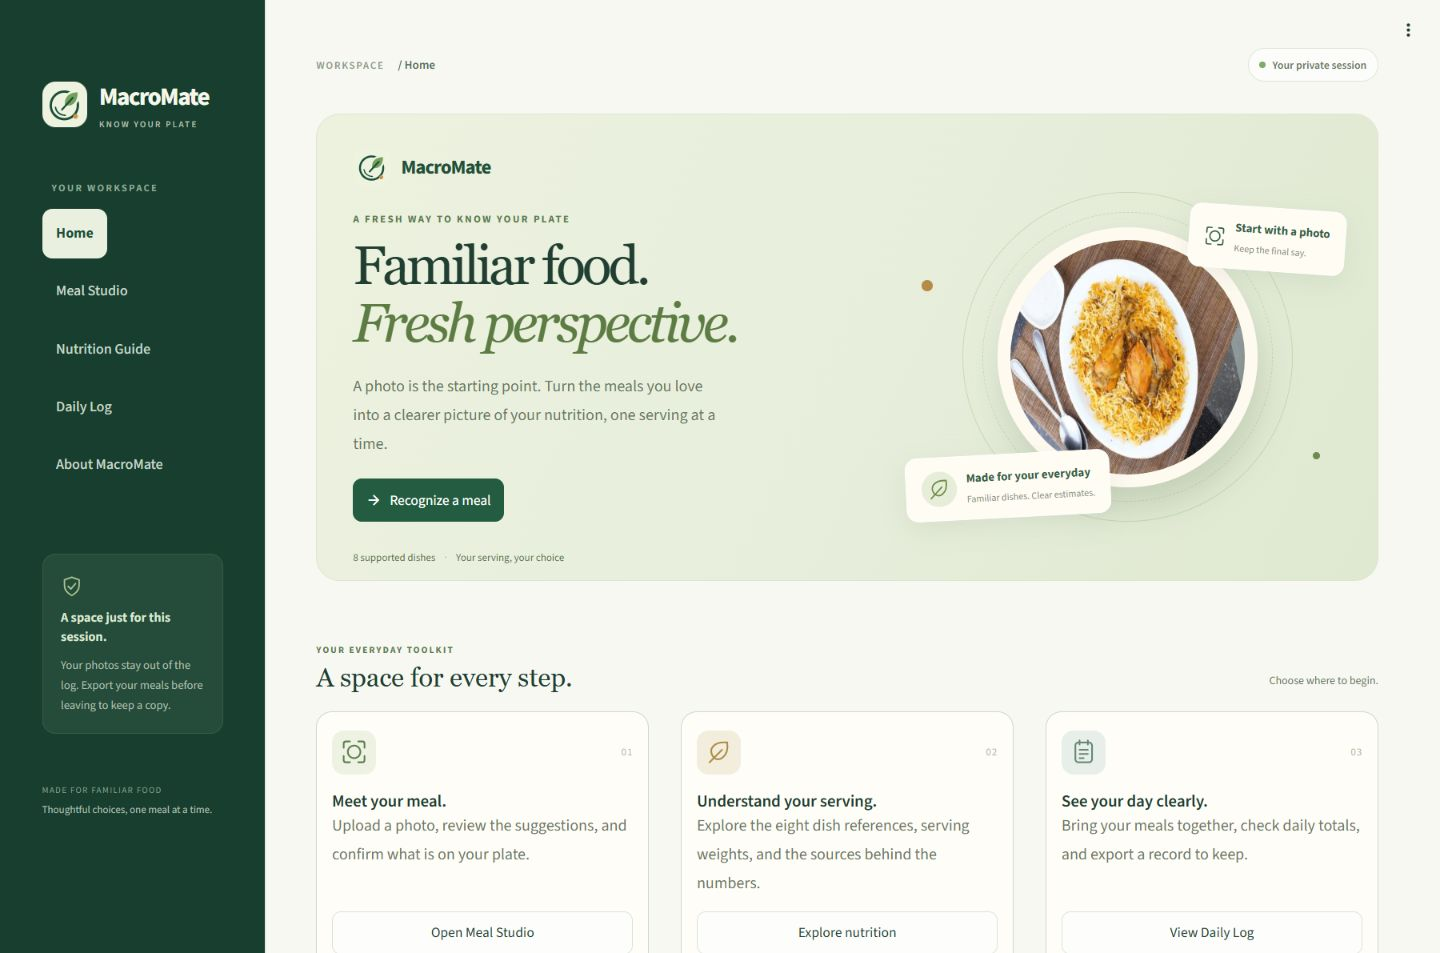
\includegraphics[width=\linewidth]{app/dashboard.png}
\caption{The redesigned branded welcome screen, captured from the local application.
The logo, main action, and three short steps introduce the meal journey.
This is UI evidence, not a model accuracy result.}
\end{figure}

\begin{center}\fbox{\parbox{.91\linewidth}{\centering
Upload JPEG/PNG $\rightarrow$ validate and decode $\rightarrow$ existing CLIP recognizer\\
$\rightarrow$ automatic suggestion $\rightarrow$ check dish and enter grams\\
$\rightarrow$ explicit confirmation and reference calculation\\
$\rightarrow$ review, save, date totals, removal/undo, and CSV export}}
\end{center}

\subsection{Upload and model integration}
Uploads are limited to 10 MB and 25 million decoded pixels. Content, not the
filename extension, determines acceptance. The Vercel entry point limits uploads
to 4 MB to fit the hosting request limit. Validation checks format, structural
integrity, full decoding, and decompression-bomb conditions before inference.
The model receives an in-memory file with \code{prepared=False}, reusing the
existing orientation/RGB/crop/normalization contract. No user photo is saved to disk.

One recognizer is reused by absolute checkpoint path, file identity, and device.
A reentrant lock serializes shared initialization and inference. Photos and
prediction results remain local to each request/session. The model-loading code
under \code{models/} and the recorded experiment evidence are preserved.

\subsection{Confirmation and state correctness}
The user can choose any of the eight supported dishes, including one outside the
top three, or select My dish isn't listed. The latter blocks estimation and
logging. Prediction never supplies serving grams. Alternate rankings, recipe
sources, and date changes are optional expandable details.

A new image clears predictions, confirmation, and estimates while preserving
already logged meals. Changing the dish requires confirmation again. Changing
grams invalidates the previous estimate. Each calculation receives one entry ID;
repeated Save operations with that ID cannot create duplicate log entries. After
saving, the UI offers My day or Add another meal. Drafts survive section changes
within the session. A new calculation intentionally creates a new entry ID.

\subsection{Nutrition calculation and assumptions}
The CSV is joined by normalized labels, never row order. Loading requires exactly
the eight unique supported labels and finite, nonnegative reference values.
Serving grams must be finite and greater than zero, with a documented 5000-g
input guard. For reference value $n_{100}$ and serving mass $m$,
\begin{equation}n(m)=n_{100}\frac{m}{100}.\end{equation}
Internal calculations and totals retain unrounded values; display and CSV export
round to two decimal places.

For chicken biryani at 150 g, the exact calculation gives 160.335 kcal, 9.945 g
protein, 21.48 g carbohydrate, and 3.135 g fat. This demonstrates arithmetic using
the committed reference, not independent validation of a photographed recipe.
Source URL, recipe assumption, source ID, and quality flag accompany the result.
Biryani uses a lower-oil reference, nihari a chicken proxy, and samosa an oven-heated
vegetable proxy. Other regional and recipe differences remain material.

\begin{figure}[htbp]\centering
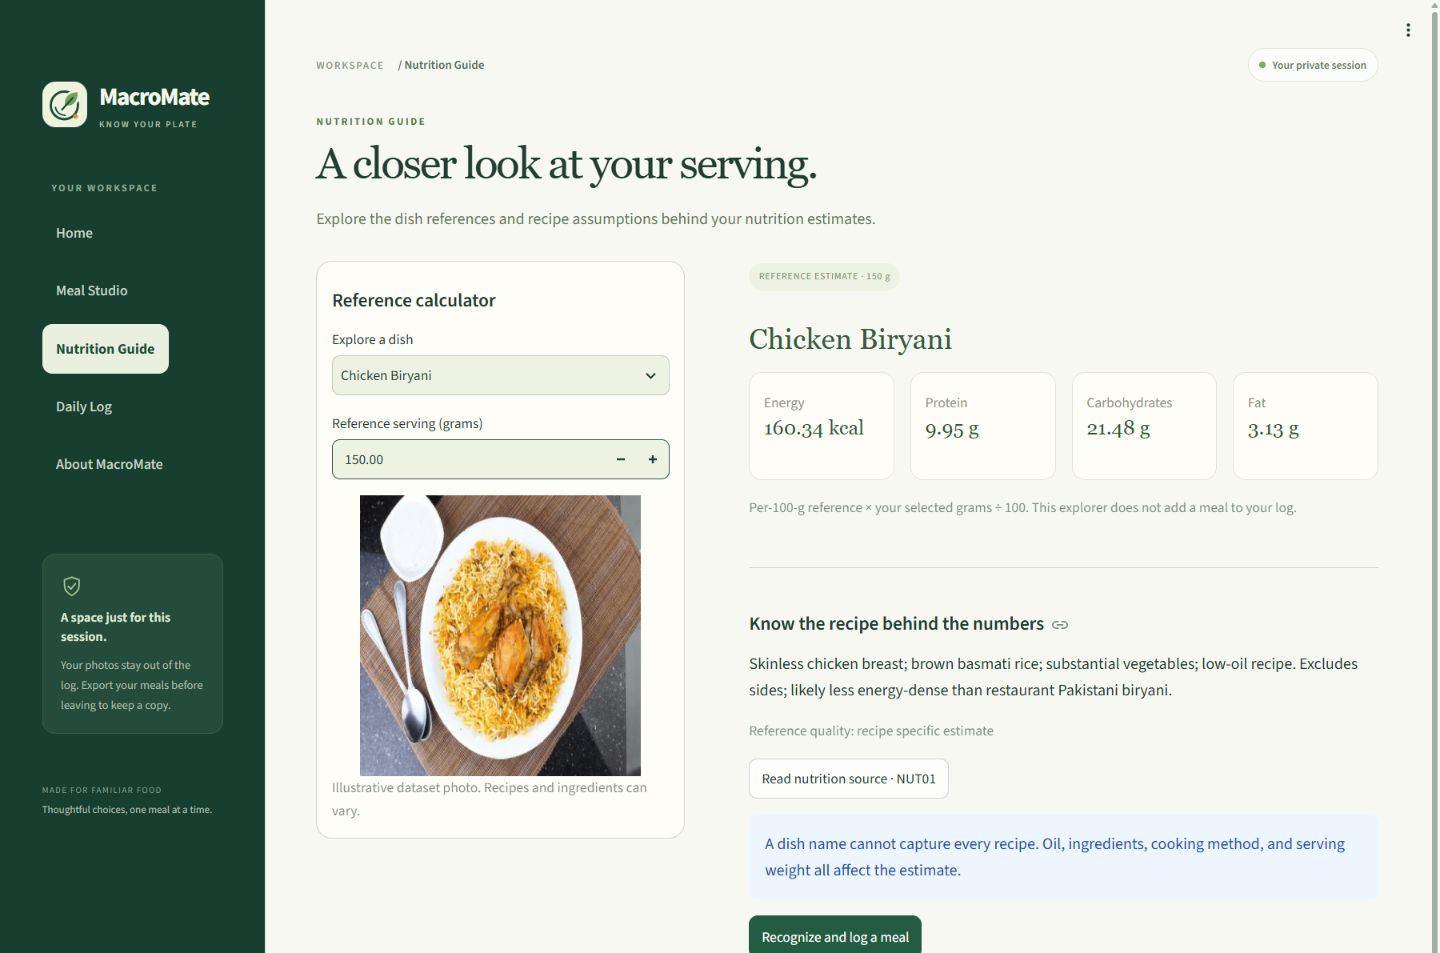
\includegraphics[width=\linewidth]{app/nutrition_guide.png}
\caption{Food guide provides an interactive reference calculator with serving
grams, optional recipe/source details, and a route back to the meal. Exploring
these values does not create a meal-log entry.}
\end{figure}

\subsection{Logging, isolation, and export}
Each session has its own \code{MealWorkflow} and \code{MealLog}. Entries contain an
ID, chosen meal date, insertion timestamp, confirmed dish, serving grams,
macronutrients, energy, and source ID. Totals filter by the explicitly selected
date. Removal uses an entry ID; Undo restores the latest removed entry with its
identity and position. Export supports the selected date or all dates.
Refresh, disconnection, hibernation, or restart can end a session; the UI states
this clearly and offers CSV export. No database or durable-storage claim is made.

\begin{figure}[htbp]\centering
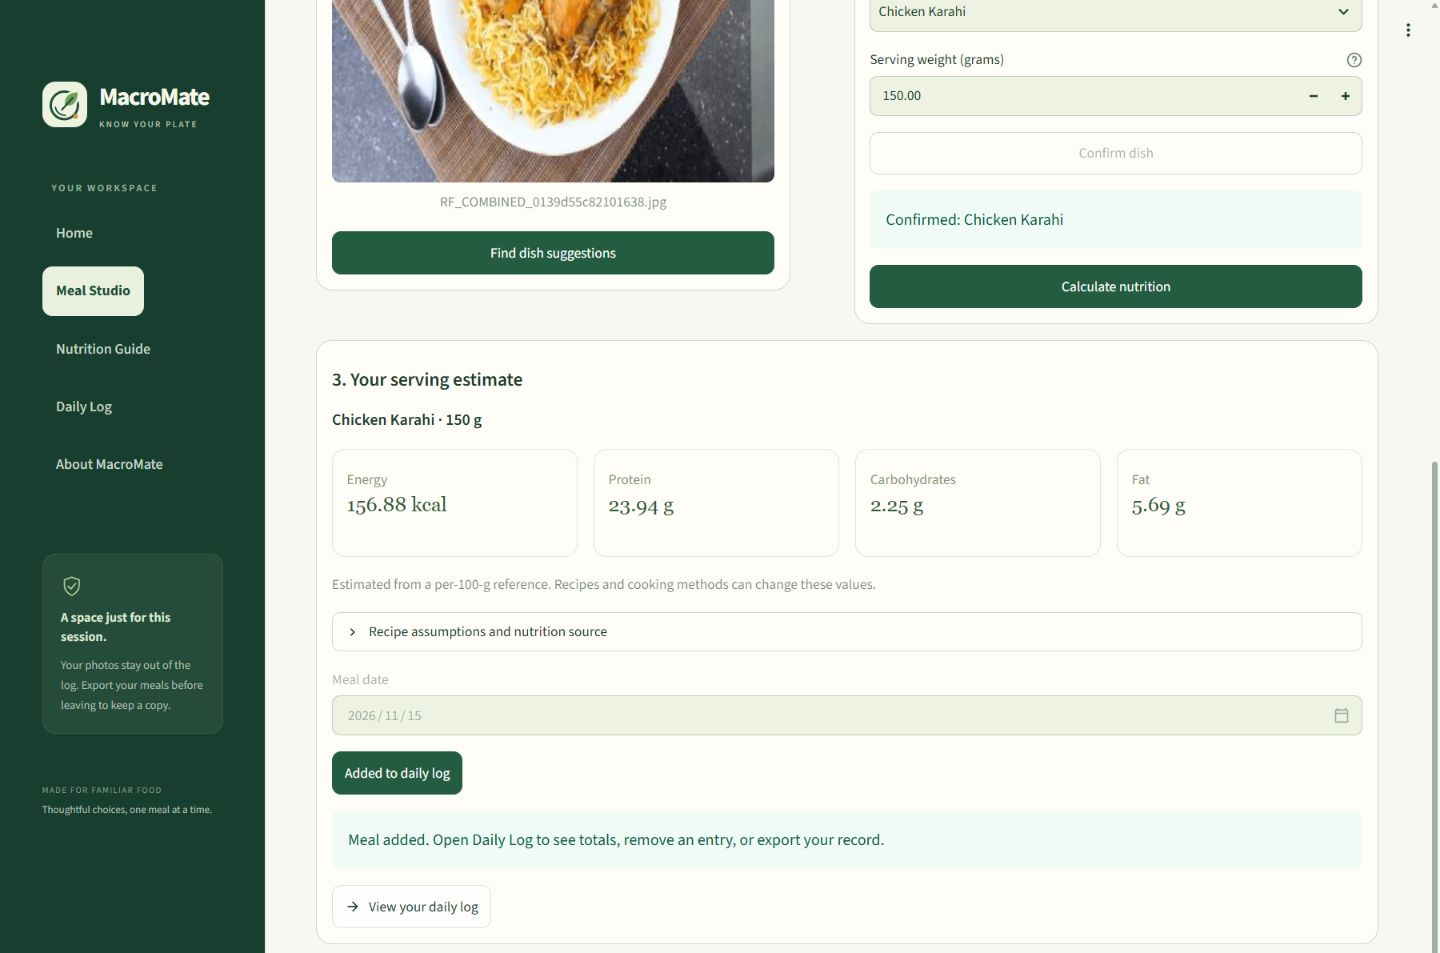
\includegraphics[width=.96\linewidth,height=.77\textheight,keepaspectratio]{app/serving.png}
\caption{Real local recognition and serving workflow. The biryani photo was intentionally
corrected to chicken karahi to test manual override; the selected 150-g reference
therefore produces 156.88 kcal. This is a functional demonstration, not a claim
that the photographed recipe has those nutrients. Photo source: Rafias Workspace,
combined-dataset; attribution remains in the manifest.}
\end{figure}

\begin{figure}[htbp]\centering
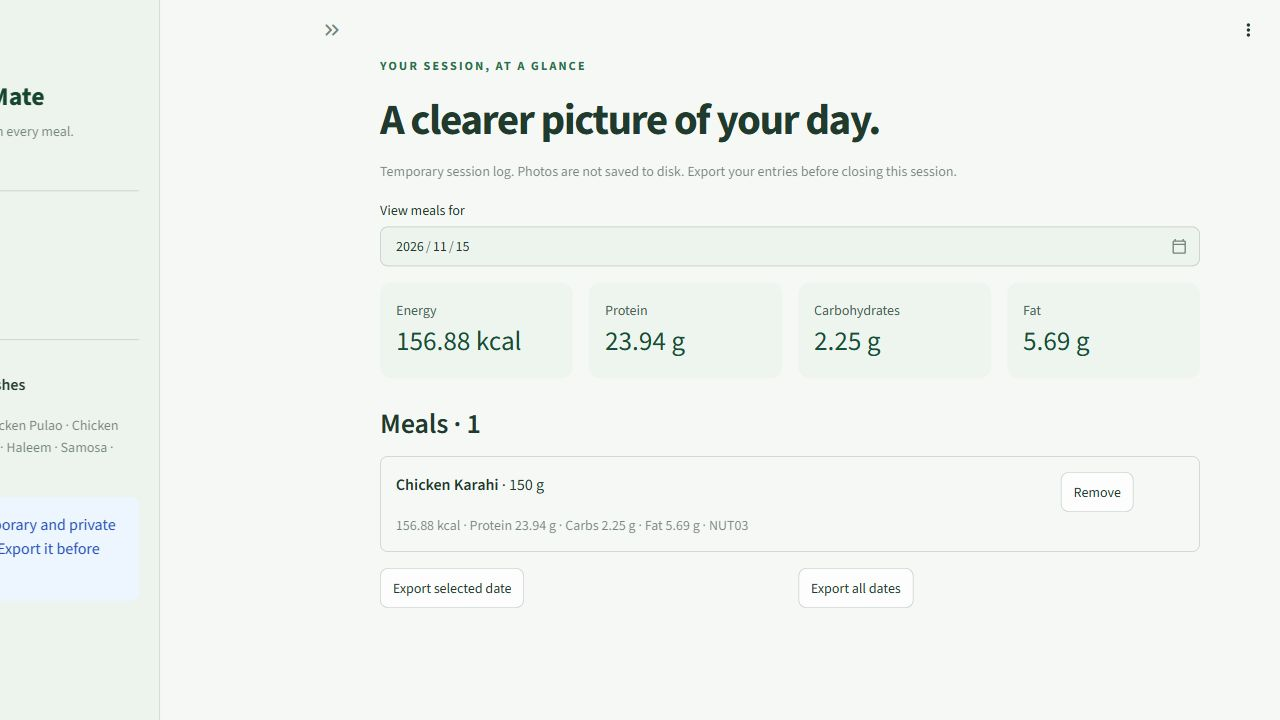
\includegraphics[width=\linewidth]{app/daily_log.png}
\caption{The same deliberately corrected meal in My day, with date totals,
removal, and CSV controls. Undo restores the entry and its totals. Source IDs
remain in exported CSV. Values demonstrate software behavior rather than independent recipe validation.}
\end{figure}

\section{Deployment and software validation}
\subsection{Reproducible deployment}
The requested target is Vercel, Python 3.12, repository-root
\code{requirements.txt}, and the ASGI entry point \code{server:app}. The wrapper
serves the same UI and limits uploads to 4 MB. Vercel configuration provisions
verified model assets at build time and requires Fluid Compute / Large Functions.
Community Cloud with \code{app.py} remains an alternative. Setup and recovery steps
are in \code{docs/deployment.md}. CPU wheels are discoverable through the official
PyTorch CPU index. Secrets are not needed for the public model assets.

The adapted checkpoint is not the full CLIP model. The setup script verifies the
released ZIP and extracted checkpoint with fixed SHA-256 values, then provisions
the pinned base cache and verifies its Git/LFS identities. A local integrity
manifest supports subsequent offline verification. All assets and downloaded
archives remain excluded from Git. The standalone UI provisions assets once per process on
the first recognition request and explains the longer initial wait.

\subsection{Validation evidence and status}
Application validation is tracked in \code{docs/deliverable3_validation.md}.
Unit tests cover arithmetic, label joins, invalid quantities, image rejection,
logging, dates, totals, CSV, and duplicate IDs. Workflow tests cover confirmation,
input invalidation, cancellation, and isolation. Streamlit AppTest exercises real
widgets with a test-only recognizer substitute; these tests do not prove actual
model execution or browser rendering.

The real-model validation script separately compares the adapter with the direct
recognizer on ten non-held-out photos and with one independent CPU CLI invocation.
It measures initialization and warm latency without retraining or rescoring the
held-out test set. Host latency, public availability, restart behavior, and
independent browser-session checks require observation of the deployed service.
Until that evidence is recorded, a prepared deployment must not be described as
a verified hosted application.

The local real-model check on 15 November 2026 passed: adapter/direct-recognizer
top-three order agreed for ten non-held-out photos, and an independent CPU CLI
invocation agreed for the selected sample. One untimed inference preceded warm
measurements. The machine used Windows 11, Python 3.12.14, PyTorch 2.9.0+cpu,
and an Intel64 Family 6 Model 126 processor. Per-photo timing, application source
hashes, checkpoint identity, and environment are retained in
\code{docs/app_validation.json}. No held-out inference was repeated.

\begin{center}\begin{tabularx}{\linewidth}{Xr}
\toprule Local software measurement & Observed result\\\midrule
Automated application tests (20 November) & 71 passed\\
Dependency consistency & No broken requirements\\
Cold model initialization (including imports) & 14.139 s\\
Warm adapter inference, median of ten & 0.148 s\\
Warm adapter inference, slowest of ten & 0.178 s\\
\bottomrule\end{tabularx}\end{center}
Downloads, UI interaction, and network latency are excluded. These figures do not
guarantee hosted performance. Hosted acceptance is recorded separately in the
release notes; these timings remain local measurements from 15 November.

A depth-one clean Git checkout also passed all 61 application tests without a
local model cache or scratch files. This check reused the verified Python
environment; public-host installation and asset downloads remain separate checks.

GitHub Actions also passed dependency installation, dependency consistency, and
the application suite on Ubuntu/Python 3.12 for application commit
\code{52cd7ae}. This Linux check uses test doubles for model calls and does not
replace the Windows real-model measurements or public deployment acceptance.
The run is linked in the validation notes.

The simplified interface passed 71 tests, including draft recovery, retry,
single-save behavior, and deployment dependency consistency. Desktop/mobile
layouts were reviewed. At \url{https://macromate-nu.vercel.app}, real-photo
recognition, manual correction, confirmation, saving, CSV export, and removal/undo
passed. The UX revision did not retrain or repeat held-out evaluation.

\section{Limitations and future work}
The main limits are the small and source-confounded collection, pending second
label review, absent external-photo evaluation, unsupported mixed plates and
unfamiliar-food rejection, uncalibrated rankings, manually estimated grams,
single-reference recipe proxies, temporary logs, and host resource limits.
Automatic serving estimation, persistent accounts, and expanded dish coverage
need separate data, design, and validation. Higher model accuracy on this same
small test set would not establish safe generalization to everyday meals.

\section{Conclusion}
MacroMate links a reproducible data/model pipeline to an explicit, reviewable
meal-logging workflow. The recorded 54/56 held-out result supports performance
on the collected test subset only. The application adds validated uploads,
manual correction, serving-based nutrition, and session-local logging with export.
Software checks and deployment evidence are kept distinct from scientific
evaluation, and readiness depends on the verified release and public-host checks.

\appendix
\section{Contribution and release traceability}
Git history records Hassan's model implementation, Mohid's image acquisition and
source records, and Adnan's cleaning, nutrition references, EDA, and initial
application backend/tests. Deliverable 3 interface, integration, validation, and
report work used AI assistance under Mohid Israr's configured Git identity.
The team retains review responsibility; historical collaboration follow-ups
remain in \code{docs/submission_checklist.md}.

\clearpage
\begin{thebibliography}{9}
\bibitem{clip} A. Radford et al. Learning Transferable Visual Models From Natural
Language Supervision. ICML, 2021. \url{https://arxiv.org/abs/2103.00020}.
\bibitem{vit} A. Dosovitskiy et al. An Image is Worth 16x16 Words: Transformers for
Image Recognition at Scale. ICLR, 2021. \url{https://arxiv.org/abs/2010.11929}.
\bibitem{streamlit-test} Streamlit. AppTest API documentation.
\url{https://docs.streamlit.io/develop/api-reference/app-testing/st.testing.v1.apptest}.
\bibitem{streamlit-cloud} Streamlit. Deploy your app on Community Cloud.
\url{https://docs.streamlit.io/deploy/streamlit-community-cloud/deploy-your-app/deploy}.
\bibitem{vercel} Vercel. Python runtime and deployment configuration.
\url{https://vercel.com/docs/functions/runtimes/python}.
\bibitem{repo} MacroMate team. Source, manifests, nutrition references, and recorded
experimental evidence. \url{https://github.com/MhassaanK68/macromate}.
\end{thebibliography}
\end{document}
